
\chapter{Background Theory}

\label{ch:background}

\section{Models of Perfect Periodic Crystal Structures}\label{perfect_periodic}
Refer to: pg 28 29 35 \cite{thin_film_Boer}\\

Theoretical models of crystalline solids are based around the existence of translational symmetry in a crystal lattice such that the lattice can be constructed by periodically repeating a unit cell of atoms. The Bravais lattice specifies the periodic array in which the repeated units of the crystal are arranged. A crystal lattice can therefore be described by its underlying Bravais lattice and the arrangement of atoms, ions or molecules within a particular unit cell, i.e. the basis \cite{AshcroftMermin2}. This principle is used in a number of ways during this study. Firstly, this process is performed on a finite scale to construct a 64 atom supercell of CZTS from the 8 atom primitive unit cell for use in density functional theory (DFT) calculations to predict defect formation energy. This process is discussed further in section \ref{supercell_section}. The principle is also used in all DFT calculations of solid state systems through the implementation of periodic boundary conditions to simulate an infinite, bulk system using only a finite unit cell.\\
 
Another important concept in the theoretical modelling of periodic structures is reciprocal space and the reciprocal lattice. 
Converting to reciprocal space enables the description of periodic features with a longer-range periodicity than the unit cell in real space, such as the motion of electrons in a crystal and phonons.
In the same way that any quantity that varies with time can be described as a sum of Fourier components in the frequency domain; the spatial properties of a crystal can be described as a sum of components in Fourier space, otherwise known as reciprocal space or \textit{k}-space. The reciprocal lattice of a perfect single crystal is an infinite periodic 3D array of points whose spacings are inversely proportional to the distances between the planes in the lattice in real space. Vectors in real space have dimensions of length, whereas vectors in reciprocal space have dimensions of length$^{-1}$. This can therefore be compared directly to the wavevector $ \left(k  = \frac{2\pi}{\lambda} \right)$ of an excitation such as a phonon or a moving electron and multiplication of each coordinate of the reciprocal lattice by $\hbar$ converts reciprocal space into momentum space as for a quantised wave $\mathbf{p} = \hbar \mathbf{k}$ \cite{Blakemore1}. \\ 

\begin{figure}[h!]
  \centering
    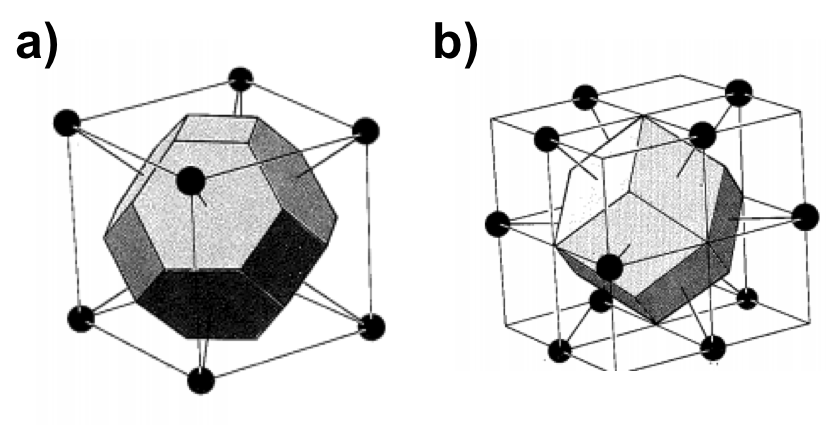
\includegraphics[width=0.5\textwidth]{figures/Wigner-Seitz.png}
    \caption{The Wigner-Seitz cell for the body-centred cubic Bravais lattice where there is a lattice point at its centre and on each vertex. The hexagonal faces bisect the lines joining the central point to the points on the vertices. The square faces bisect the lines joining the central point to the central points in each of the six neighbouring cubic cells. Figure taken from reference \citenum{AshcroftMermin2}.}
  \label{Wigner-Seitz}
\end{figure}

The Wigner-Seitz primitive cell is the most common choice of primitive cell with the full symmetry of the Bravais lattice. It represents the region of space around a lattice point  that is closer to that point than to any other lattice point. For example, figure \ref{Wigner-Seitz}a shows the truncated octahedron that is the Wigner-Seitz cell for a body-centred cubic (bcc) lattice \cite{AshcroftMermin2}.
The first Brillouin zone is the Wigner-Seitz primitive cell of the reciprocal lattice. The reciprocal of the bcc lattice is face-centred cubic (fcc), therefore the first Brillouin zone of  of the bcc lattice is the fcc Wigner-Seitz primitive cell as shown in figure \ref{Wigner-Seitz}b \cite{AshcroftMermin3}. As the full symmetry of the reciprocal lattice is contained within the first Brillouin zone, it is only necessary to sample \textit{k}-points within this single unit cell of the reciprocal lattice when calculating the electronic ground state of a periodic structure.

 
\section{Band Theory \& Band Structure of Semiconductors}\label{band_theory}
Refer to: pg 18 \cite{fund_semi}, pg 105 112 128 131 137 \cite{thin_film_Boer}, pg 111 + 119 \cite{phys_semicond}\\

** Highlight link to PV and indication of PV performance from band structure + check against Nelson CH3\\

The band theory of solids provides a means to explain the difference in the electrical conductivity of conductors, semiconductors and insulators. Electrons bound to an atom have a number of possible discrete energy levels. When a large number of atoms are brought together to form a solid, it becomes impossible to assign individual electrons to individual atoms. Instead, the electrons are considered to be shared amongst the atomic nuclei. However, a consequence of this sharing would be a large number of electrons occupying the same energy state, which violates the Pauli Exclusion Principle. The original discrete energy levels therefore are broadened into bands. The new energy levels are so closely spaced that they are considered to be a quasi-continuous band of allowed energies. This is illustrated in figure \ref{band_Elevels}. The series of bands of allowed energies in a semiconductor or insulator are separated by bands of forbidden energy, known as the band gap, E$_g$, of the material \cite{dielectric1}. In the simplest model, the upper energy band (the conduction band) is separated from the lower energy band (the valence band) by a constant band gap, which was discussed in section \ref{PV_properties} for the important role this optical property has in a solar absorber material. This is called the flat band model and is often shown in schematics of p-n junctions for PV devices, such as in figure \ref{PV_schematic}. In real structures, the band architecture is more complicated than this simple model, like the band structures shown in figure \ref{Si_and_GaAs} \cite{Tilley}.\\

\begin{figure}[h!]
  \centering
    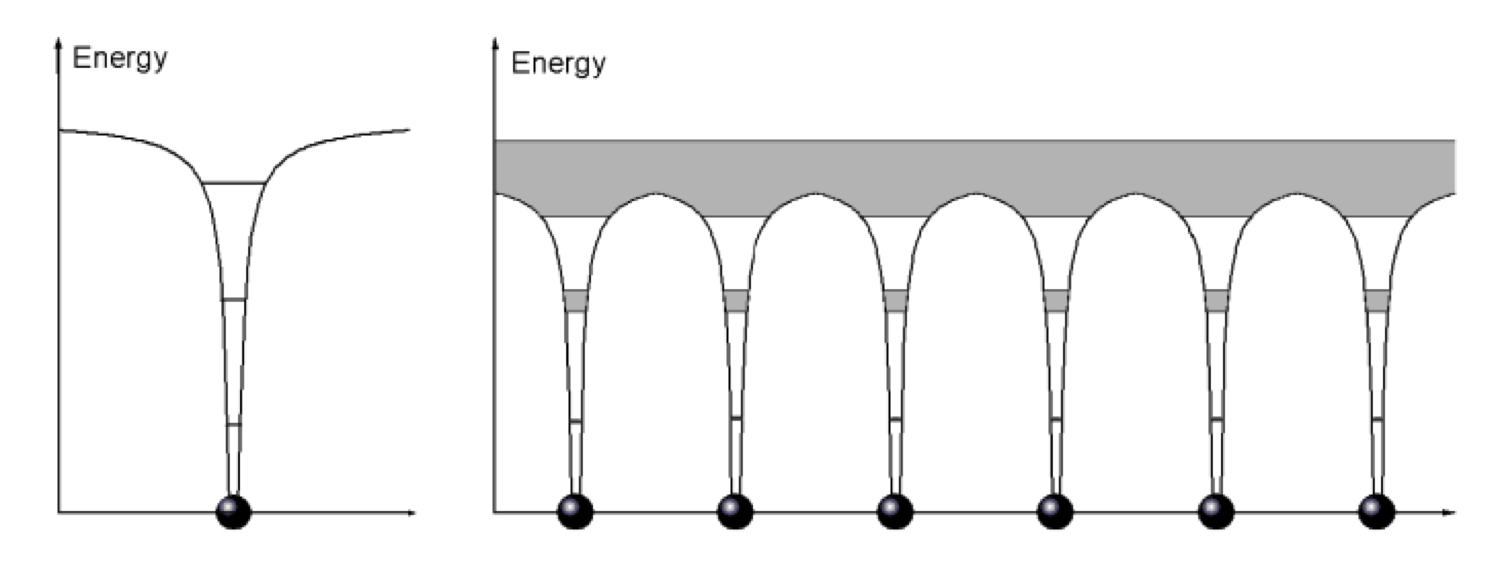
\includegraphics[width=0.7\textwidth]{figures/band_Elevels.png}
    \caption{Electron energy levels of a single atom (left) and the formation of a quasi-continuous band of allowed energies in a solid crystal when many atoms are brough close together (right). Figure taken from \citenum{mat_prop1}.}
  \label{band_Elevels}
\end{figure}

The concept of the energy band model of a solid emerges from considering the behaviour of electrons in a periodic crystal lattice, but cannot be understood in terms of classical physics alone. Instead, the electron must be considered in terms of wave-mechanical terms as a wave propagating in a periodic structure with diffraction and interference effects  \cite{small_semiconductor1}.
In the band theory of 
solids, the energy of a single electron in a perfect crystal is described by the one-electron Schr{\"o}dinger equation, shown in equation \ref{single_SE}. The first term in equation \ref{single_SE} is the kinetic 
energy of the electron, V(\textbf{r}) is the effective non-zero periodic potential energy experienced by 
the electron in the crystal, $\psi$ is the electron wavefunction and  $\epsilon$ is the eigenenergy of the electron. In band theory, it is assumed that for any electron, everything else in the crystal can be represented by the effective potential energy, V(\textbf{r}) \cite{Blakemore2}.
\begin{equation} \label{single_SE}
\left[ \left(-\frac{\hbar^2}{2m}\right)\nabla^2 + V(\mathbf{r})\right]\psi = \epsilon \psi 
\end{equation}
The spatial dependence of the potential experienced by an outer electron in a crystal for multi-electron systems was considered by Felix Bloch. He determined that the total potential is the sum of two parts. Firstly, the electrostatic potential due to the array of atomic cores. For a perfect lattice this should have the translational periodicity of the lattice. Secondly, the potential due to all other electrons. Bloch assumed that the charge density would have the same long-term average value in every unit cell of the crystal and therefore would be periodic. Bloch's theorem states that the wavefunction which satisfies equation \ref{single_SE} subject to a periodic potential should be of the form shown in equation \ref{bloch}, where $U_k(\mathbf{r})$ is some function 
(depending on the value of the wavevector, \textbf{k}) that also has the complete 
periodicity of the lattice and \textbf{k} is confined to the first Brillouin zone \cite{Blakemore2}.
\begin{equation} \label{bloch}
\phi_k(\mathbf{r}) = U_k(\mathbf{r}) e^{i\mathbf{k \cdot r}} 
\end{equation}
\begin{equation} \label{bloch_sum}
\psi_k(\mathbf{r}) = \sum_k A_k \phi_k(\mathbf{r}) = \sum_k A_kU_k(\mathbf{r}) e^{i\mathbf{k \cdot r}} 
\end{equation}
Due to the translational symmetry of a crystal lattice, an eigenfunction of the one-electron Schr{\"o}dinger equation can be expressed as a sum of Bloch functions such as that shown in equation \ref{bloch}, as shown in equation \ref{bloch_sum}. The one-electron wavefunctions therefore can be indexed by constants \textbf{k}, which are the wave vectors of the plane waves forming the `backbone' of the Bloch function. A plot of the electron eigenenergies from equation \ref{single_SE} versus \textbf{k} is known as the electronic band structure of the crystal \cite{fund_semi}.\\

\begin{figure}[h!]
  \centering
    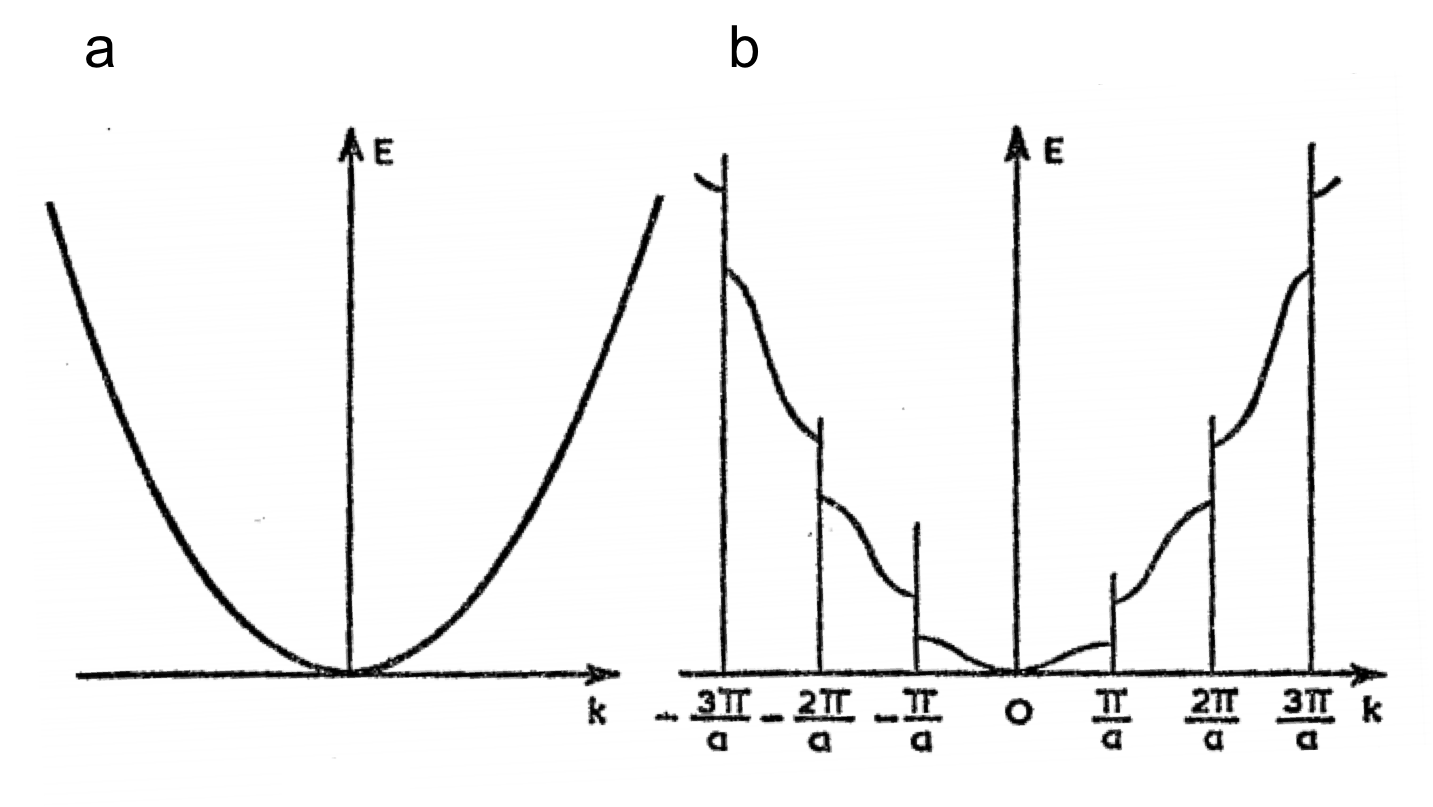
\includegraphics[width=0.7\textwidth]{figures/bs1.png}
    \caption{Energy-wave vector diagrams: (a) the free electron parabola, (b) modification due to a periodic crystal lattice. Figure taken from reference \citenum{small_semiconductor1}.}
  \label{bs1}
\end{figure}

The introduction of a medium with a discrete structure, such as a crystal lattice, has a profound effect on the dispersion relation of the waves. The energy dispersion relation of a free electron and that in a periodic crystal lattice is shown in figure \ref{bs1}. A periodic medium does not completely suppress the propagation of waves, as would be expected  in disordered or amorphous structures, but they do however introduce limiting frequencies and wavelengths for the propagation, followed by cut-off regions. The lower limit of the wavelength is set by the lattice spacing, a, giving an upper limit of the wave vector, \textbf{k}, of $\frac{\pi}{a}$. As figure \ref{bs1} shows, the parabola of the free electron in modified in a periodic crystal by the introduction of discontinuities at values of \textbf{k} corresponding to multiples of $\frac{\pi}{a}$. The appearance of such energy gaps implies that electrons in a periodic crystal may only have kinetic energies corresponding to certain bands, whilst being free to propagate in the lattice \cite{small_semiconductor2}.\\

Each electron occupies a state of definite $\mathbf{k}$. Therefore, an infinite number of electrons within the solid would result in an infinite number of \textit{k}-points. At each \textit{k}-point, only a finite number of the available energy levels will be occupied. Therefore only a finite number of electrons need to be considered but at an infinite number of \textit{k}-points. In practise, all of these \textit{k}-points are not considered. 
Electron wavefunctions will be almost identical for values of $\mathbf{k}$ that are sufficiently close, so the wavefunctions over a region of reciprocal space can be represented by considering the wavefunction at a single \textit{k}-point. It is therefore sufficient to consider the electronic states at a finite number of \textit{k}-points in order to determine the ground state energy of the solid. This approximation is illustrated in figure \ref{energy_dispersion}. Using Bloch's Theorem therefore has enabled the ground state energy to be determined by considering only the number of electrons in the unit cell at a finite number of \textit{k}-points, which are chosen to sample the Brillouin zone appropriately. The choice here is a balance between more \textit{k}-points for a more accurate representation of the Brillouin zone and fewer \textit{k}-points to reduce the computational expense of the calculation \cite{bloch-thesis}.\\

\begin{figure}[h!]
  \centering
    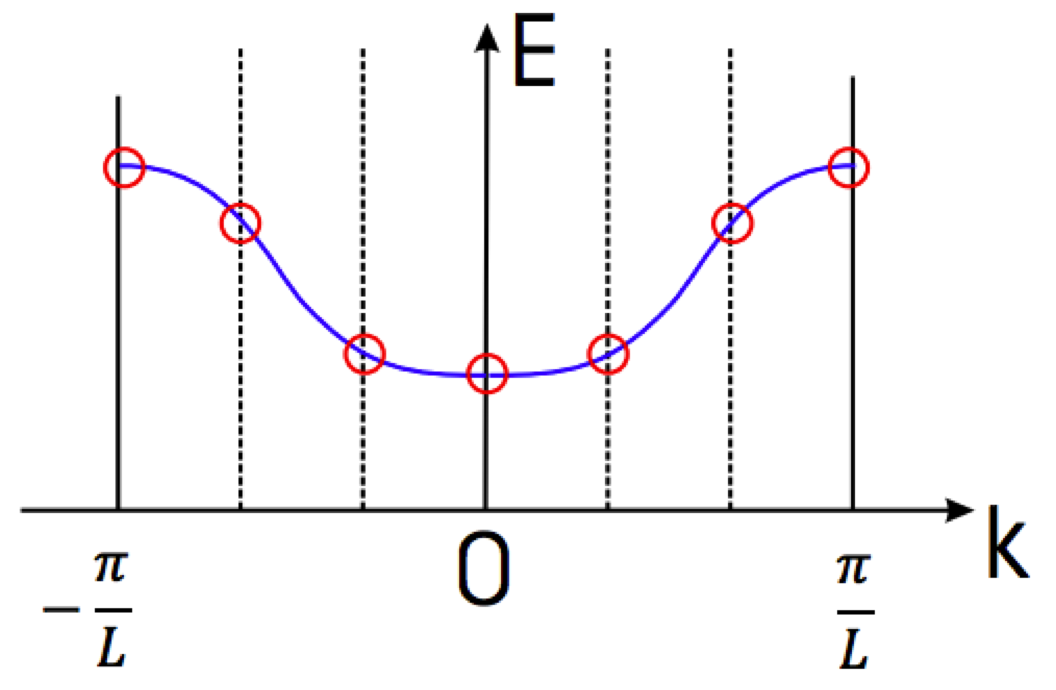
\includegraphics[width=0.4\textwidth]{figures/energy_dispersion.png}
    \caption{The energy dispersion relation for electrons moving in a crystal, illustrating how the function can be approximately represented by a finite number of \textit{k}-points, which form an equally-spaced mesh. Figure adapted from reference \citenum{vasp-slides}.}
  \label{energy_dispersion}
\end{figure}

A useful concept used to simplify the dynamics of an electron in a crystal lattice in the band theory of solids is that of effective mass, which was first mentioned in section \ref{PV_properties} as a key material property for a solar absorber material. The effective mass is a convenient parameter which accounts for the influence of a periodic lattice on a free carrier, enabling an electron in a periodic crystal to be treated as though it were a free particle but with a different mass in calculations of charge transport. Values of effective mass in semiconductors usually vary between 0.01 and 1 times the mass of a free electron and it is determined by the curvature of the energy graph in \textit{k}-vector space \cite{small_semiconductor2}. The effective mass is a parameter that can influence the efficiency of a solar cell, in particular, the effective mass of holes in the valence band and electrons in the conduction band (i.e. minority charge carriers) are of interest. The mobility of charge carriers is inversely proportional to the effective mass and the mobility of charge carriers in a PV material is important for efficient charge collection \cite{transport}.
 
 
% \section{Vibrational Properties of Semiconductors \& Electron-Phonon Coupling}
 
 %**mention short diffusion length of CZTS compared to other technology\\
 
%In section \ref{PV_properties}, both effective mass and dielectric function were discussed for the insight these properties can provide for the likely PV performance of a material due to the impact these properties can have on the mobility of charge carriers in that material. However these are certainly not the only features of a real material at finite temperatures that need to be considered to understand carrier mobility in a material. 
%Even in a perfect crystal, atoms are involved in some sort of thermal motion about their idealized equilibrium positions. The simplest model to describe this motion is the Einstein model where each atom vibrates independently and as a simple harmonic oscillator in the potential well created by the force fields of its neighbouring atoms. The field can never be precisely a quadratic well with spherical symmetry, but on average the approximation is reasonable, especially when only only a very crude picture of thermal vibrations is sufficient or at fairly high temperatures, when the assumption that atoms vibrate independently of each other is more justified \cite{Ziman_solids}. In this model, the oscillations of the atoms can be expressed in terms of normal modes as they are independent of each other. Energies of these normal modes are then quantised, where a quantum of lattice vibration is referred to as a phonon \cite{fund_semi}.\\

%\begin{figure}[h!]
%  \centering
%    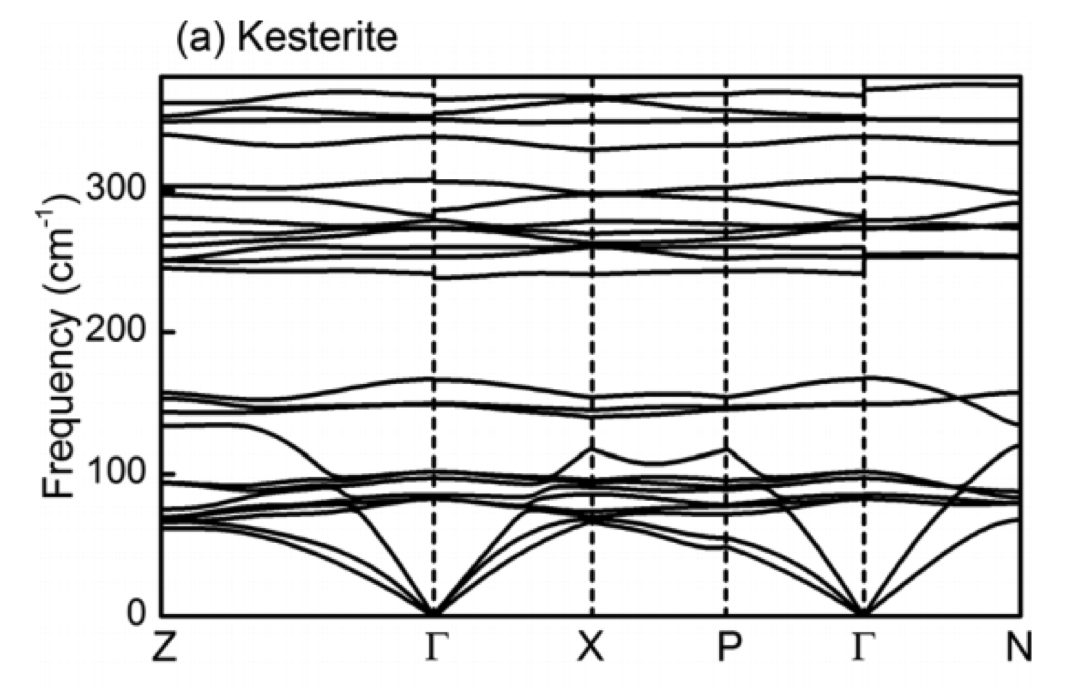
\includegraphics[width=0.9\textwidth]{figures/CZTS_phonons.png}
%    \caption{Phonon dispersion curve of {\CZTS} and DOS... Figure taken from %\citenum{CZTS_phonons}.}
 % \label{defects}
%\end{figure}

%three of which are lower-energy acoustic branches and the rest are optical curves??

%For a given crystal structure, there are 3N phonon modes, where N is the number of atoms in the primitive unit cell. In the case of {\CZTS}, there are therefore 24 phonon modes. The phonon dispersion curves for kesterite-structured {\CZTS} and associated density of states are shown in figure \ref{CZTS_phonons}.
%Along directions of high symmetry these phonons can be classified as transverse or longitudinal depending on whether their displacements are perpendicular or parallel to the direction of the wavevector respectively. In a solid the long wavelength transverse acoustic (TA) phonons are shear sound waves, while the longitudinal acoustic (LA) phonons are compressional sound waves. The velocities of these sound waves are determined by shear and bulk elastic moduli respectively. As it is usually easier to shear than to compress a crystal, TA phonons typically travel with lower velocities than LA phonons.  
%The atomic displacements from long wavelength acoustic phonons can correspond to a deformation of the crystal, this is referred to as deformation potential theorem. Such deformations will change the electronic energies at different points in the Brillouin zone. LA phonons always produce a change in the volume of the crystal, which affects all energy bands \cite{fund_semi}.\\

%The interaction of charge carriers with phonons, often referred to as electron-phonon coupling, sets a fundamental limit on the mobility of charge carriers in a material in the absence of extrinsic scattering due to defects, impurities or interfaces \cite{fund_semi, MAPI_Eg_broadening}. 
%{\CZTS} in particular has been shown to have a low carrier diffusion length compared to other absorber materials **FIND REF**.
%Thermal vibrations of the lattice atoms gives rise to a perturbation of the band edge \cite{thin_film_Boer}, although the interaction of charge carriers with phonons is currently still a subject of much debate \cite{MAPI_Eg_broadening16, MAPI_Eg_broadening17, MAPI_Eg_broadening}.
%Of all the various possible contributions to intrinsic band gap broadening from electron-phonon coupling, there is currently no clear picture of which mechanisms are active or the most dominant in determining the carrier mobility in a material \cite{MAPI_Eg_broadening}, however it could be argued that lowest energy phonon modes are likely to make the biggest contribution. A number of studies on non-polar inorganic semiconductors have examined the temperature dependence of the charge-carrier mobility \cite{MAPI_Eg_broadening21, MAPI_Eg_broadening22, MAPI_Eg_broadening23, MAPI_Eg_broadening24}, where the carrier mobility, $\mu$, was found to scale with $T^m$ where m has a value between -1.4 and -1.6. From theory, it is known that deformation potential scattering with acoustic phonons results in $\mu \propto T^{-\frac{3}{2}}$. Therefore several works in the literature suggest that electron-phonon coupling at room temperature is dominated by acoustic phonons \cite{MAPI_Eg_broadening16, MAPI_Eg_broadening17, MAPI_Eg_broadening24}. Looking again at figure \ref{CZTS_phonons}, the acoustic modes are the three that tend to zero at the gamma point.
%In our study, we will first be determining just the contribution from LA phonons due to the changes in lattice volume from to the thermal motion of the atoms in an attempt to gauge if the fundamental limit this places on carrier mobility is likely to be a key limiting factor for device performance. The carrier lifetime in CZTS has been measured to be considerably less than that of other technologies (e.g. MAPI)... **FIND REF** The methodology for this calculation will be discussed in section \ref{band_gap_broadening}.
 
\section{Electronic Properties of Defects in Semiconductors}
%Refer to: pg 160 \cite{fund_semi}, pg 51, 52, 64 \cite{thin_film_Boer}, pg 63 + 65 \cite{phys_semicond}\\

Check against Aron's concise theory of pt defects on group wiki?\\

Although the main framework for materials modelling of solid-state systems (as was outlined in section \ref{perfect_periodic}) is built around perfect, periodic systems; in reality absolutely perfect systems do not exist. There is an energy cost associated with the creation of a defect, but in many cases the free energy of a system can be lowered by the incorporation of a certain concentration of defects due to an increase in the configurational entropy of the system \cite{AshcroftMermin_general}. 
At this point it is worth distinguishing between different types of defects for the purpose of later discussions.
Firstly, if a defect does not involve any atoms that are foreign to the host crystal, then the defect is called an intrinsic or native defect. Defects involving foreign atoms, or impurities, are referred to as extrinsic defects. Figure \ref{defects}a and \ref{defects}b show some examples of extrinsic and intrinsic defects. In our study on {\CZTS} as we are first interested in the fundamental material properties so we are currently only concerned with intrinsic impurities, although in real systems impurities are often unintentionally present in the growth or processing environment.
Defects are usually classified as point or line defects. Point defects usually involve isolated atoms in localized regions of a host crystal, whereas line defects involve rows of atoms, such as a dislocation defect. An example of a line defect is shown in figure \ref{defects}a. Another possible type of defect is a defect complex, which is composed of a small number of point defects. Some examples of defect complexes in {\CZTS} were shown in figure \ref{Chen_cluster1}. Defect complexes can be particularly interesting to study as there is some speculation in the literature that defects which are energetically less likely to form, could be more likely to form if they form a defect complex with defects that are more likely to form **find ref**.
There are then a number of different possible point defects, such as: vacancies, interstitials and antisites. In the case of our study on defects in {\CZTS}, it is sulfur vacancies ($V_{S}^{0}$, $V_{S}^{+}$, $V_{S}^{2+}$) and copper-on-zinc ($Cu_{Zn}^{-}$) and zinc-on-copper ($Zn_{Cu}^{+}$) antisites that are of interest, where  $Cu_{Zn}^{-}$ and $Zn_{Cu}^{+}$ form the charge neutral defect complex [$Cu_{Zn}^{-}$ + $Zn_{Cu}^{+}$]. The sulfur vacancy is an example of an electrically active defect. In this case the defect can contribute two free electrons to the host crystal and so is a donor or n-type defect.
**check** The free electrons can then either be fairly localized on the defect site to form a small polaron, or extended across several sites to form a large polaron, or be completely delocalized across the system **find ref**.\\

\begin{figure}[h!]
  \centering
    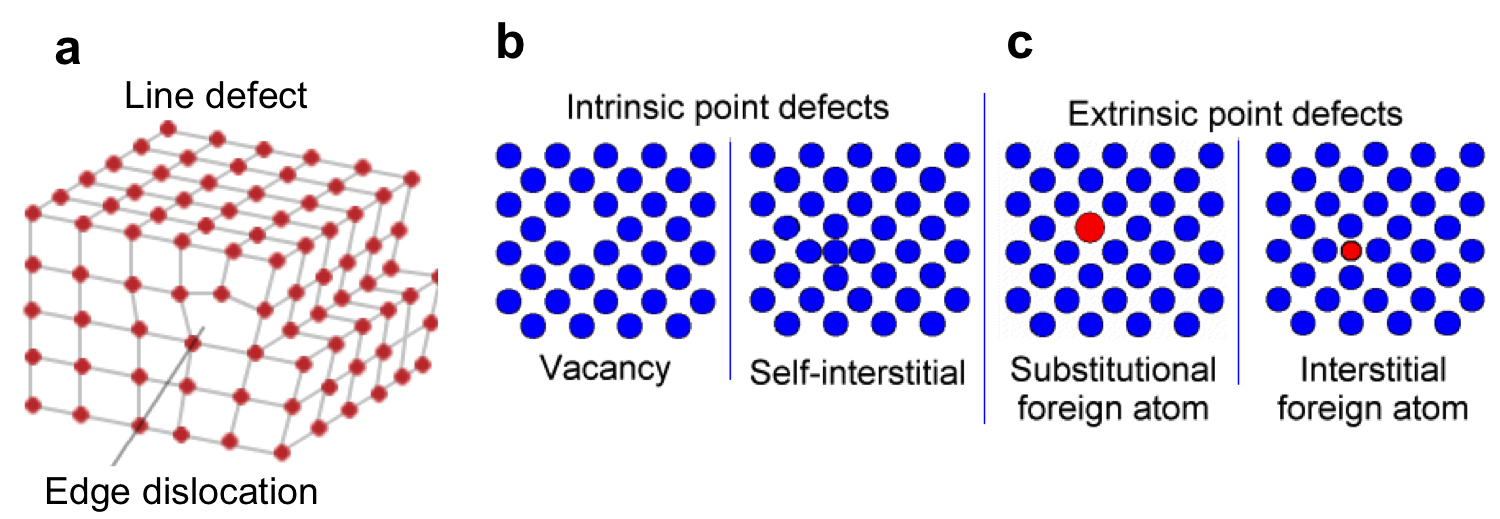
\includegraphics[width=0.9\textwidth]{figures/defects.png}
    \caption{An example of a line defect (a) and both intrinsic (b) and extrinsic (c) point defects. Figures taken from references \citenum{defects_fig1} and \citenum{defects_fig2} respectively.}
  \label{defects}
\end{figure}

The electrical properties of semiconductors can be modified significantly by the incorporation of very small amounts of impurities or defects. It is often the case that less than one defect per million of host atoms is sufficient to alter the properties of a semiconductor \cite{fund_semi}. This sensitivity to defects is one of the reasons why semiconductors find many uses in device applications. For example, luminescence centres in wide-band-gap materials can be used to emit light at specific wavelengths or single-spin centres provided by defects can act as artificial atoms and serve as a qubit in a quantum information system \cite{defects_tutorial}. In order to control the electrical properties of a material by introducing defects, typically processes must first be developed to produce a fairly defect-free material, before intentionally introducing particular defects \cite{fund_semi}. However in the case of solar cell devices the presence of defects is typically detrimental. Various ways in which defects in the absorber material can impede solar cell performance are discussed further in section \ref{defects_in_PV} and more general characteristics of defects in semiconductors are discussed in the next section.

%\begin{itemize}
%\item Notes from A. Guinier 'X-Ray Diffraction' CH6 + Ziman
%\item Mention many types of disorder possible for multicomponent, especially for multi-component, compound semiconductor. e.g. of many types of possible defects for CdTe from Ken's work - and that's just binary!
%\item Extended defects usually detectable? 
%\item Discuss frozen in disorder and Scragg's work?
%\end{itemize}



\subsection{Impact of Defects on the Band Structure \& Optical Spectra}\label{PL_section}
The energy band model, which was discussed in section \ref{band_theory}, has been successful in explaining many aspects of the behaviour of solids and a large amount of experimental data collected has supported the theoretical predictions made using the model. Its main drawback however is that it assumes a perfect, or nearly perfect, crystal lattice. It applies well to single crystals and polycrystalline substances, but cannot be applied to materials that are amorphous or heavily disordered so that the structure deviates significantly from the periodicity of the crystal \cite{small_semiconductor1}. \\

Some defects result in additional energy levels in between the valance-band maximum and conduction-band minimum, i.e. within the band gap of the material. Electrically active defects have at least one defect level in the band gap. This level then has an associated defect wavefunction, a state to which the electron is added to or removed when the charge state of the defect changes. If the defect level is positioned relative to the band edges such that the defect is likely to be thermally ionized at room temperature then the defect is conventionally referred to as a shallow level. Otherwise it is a referred to as a deep level. Typically deep levels are thought to be the most detrimental to solar cell device performance, which will be discussed further in section \ref{defects_in_PV}. Another way of defining a defect as `shallow' or `deep' is based on the degree of localization of the wavefunction. If a defect wavefunction is delocalized (on the order of many lattice constants) then the defect has the characteristics of a shallow defect. If the wavefunction is instead localized on the length scale of an atomic bond then this indicates a deep level defect \cite{defects_tutorial}.\\

\begin{figure}[h!]
  \centering
    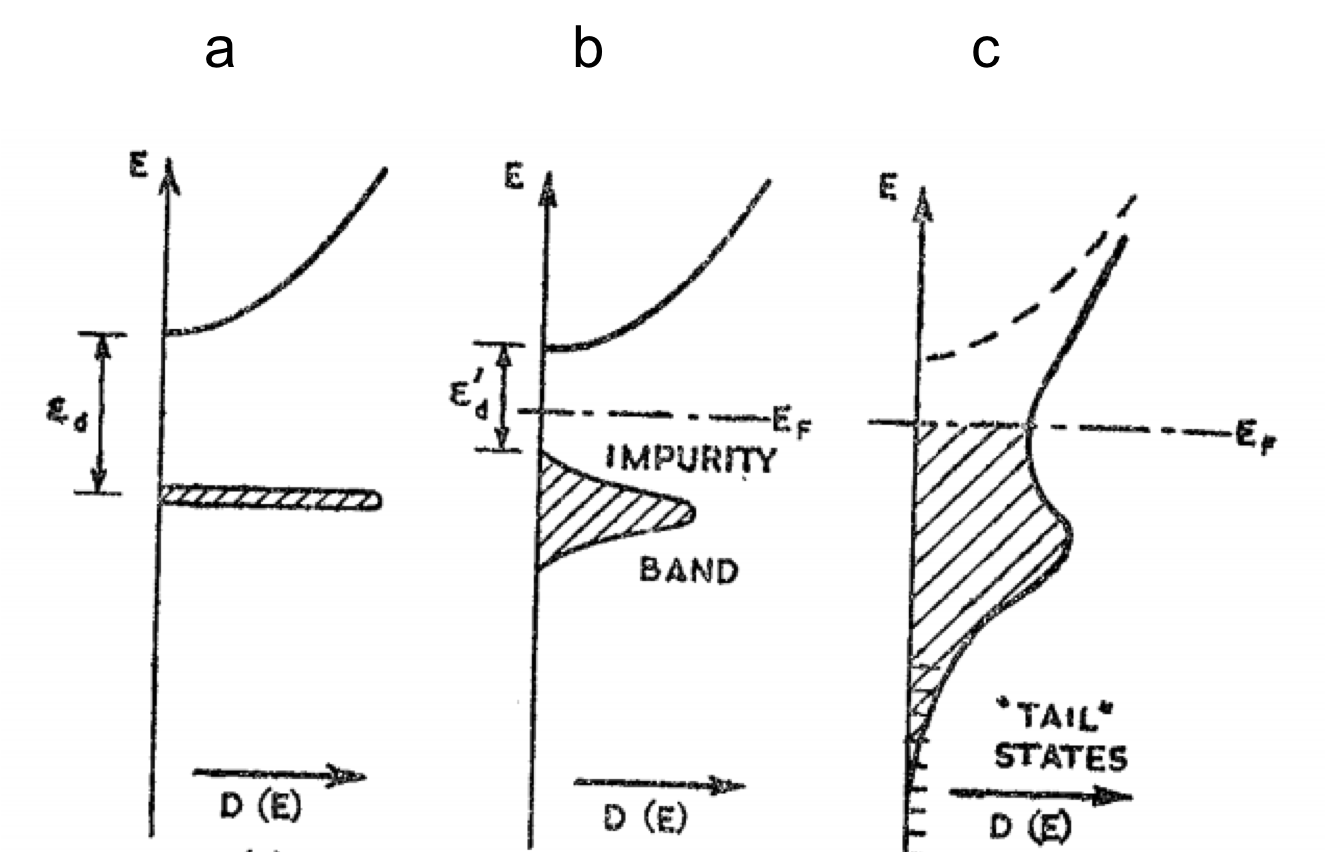
\includegraphics[width=0.7\textwidth]{figures/bs2.png}
    \caption{The influence of increased donor impurity density on the conduction band profile showing low (a), medium (b) and high (c) densities of impurities. Figure taken from reference \citenum{small_semiconductor2}.}
  \label{bs2}
\end{figure}

Low concentrations of impurities and defects can be modelled by considering, for example, the introduction of distinct additional donor and acceptor energy levels within the band gap of a material and the scattering of electrons and holes in the solid. However, at higher defect concentration, these local levels interact to form a band. For high n-type doping, for example, the impurity band merges with the conduction band, causing a rigid shift of the conduction band towards the valence band \cite{Pankove}. The band profile can be modified with increasing donor density as shown in figure \ref{bs2} to give rise to conductivity even at temperatures that are too low to produce excitation of carriers into the free conduction bands, called impurity band conduction \cite{small_semiconductor2}.
In heavily-doped semiconductors it is possible to observe a phenomena called `band tailing', where the valence and conduction bands are shifted towards each other resulting in a narrowing of the band gap, as shown in figure \ref{pankove_band_tailing} \cite{Pankove}. The heavy-doping effects then result in a different emitted spectrum which can be detected by techniques such as photoluminescence (PL) spectroscopy. \\

\begin{figure}[h!]
  \centering
    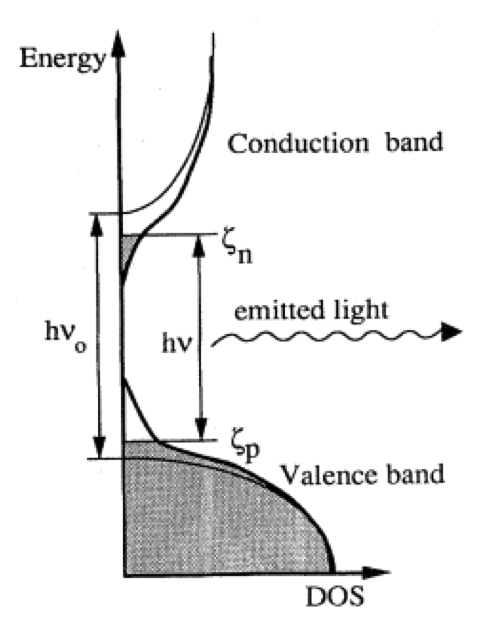
\includegraphics[width=0.4\textwidth]{figures/pankove_band_tailing.png}
    \caption{Schematic of the laser operation at T=0 K in GaAs. $\zeta_{n,p}$ are the quasi-Fermi level for electrons and holes respectively. The narrow line denotes the unperturbed DOS, while the heavy line depicts the DOS modified by heavy-doping effects. Both valence and conduction bands are shifted towards each other to give a narrowing of the band gap and the DOS is distorted, showing band tails. Heavy doping effects result in a different emitted spectrum. Figure taken from reference \citenum{Pankove}.}
  \label{pankove_band_tailing}
\end{figure}

In a PL experiment, photons with energies larger than that of the band gap excite electrons from the valence band to the conduction band, as shown in figure \ref{PL_transitions}a. In addition, electrons can be excited from or to defect levels, as shown in figure \ref{PL_transitions}b. When the excited electrons transition to lower energy levels, they can emit light to conserve energy, resulting in a peak in the PL spectrum. In a photoluminescence excitation (PLE) experiment, the PL intensity is measured as a function of excitation photon energy. This gives an absorption profile for the defect. PL measurements are able to pick up optical signatures of defects even if they are only present at low concentrations with high resolution \cite{defects_tutorial}. A review of some of the photoluminesence spectra for {\CZTS} in the literature and the implications for PV device performance is discussed in section \ref{CZTS_PL_section}. PL measurements alone however cannot be used to identify the character of a defect, this is an area where first-principles defect calculations (which are discussed in the methodology section) can provide valuable insight \cite{defects_tutorial}.

\begin{figure}[h!]
  \centering
    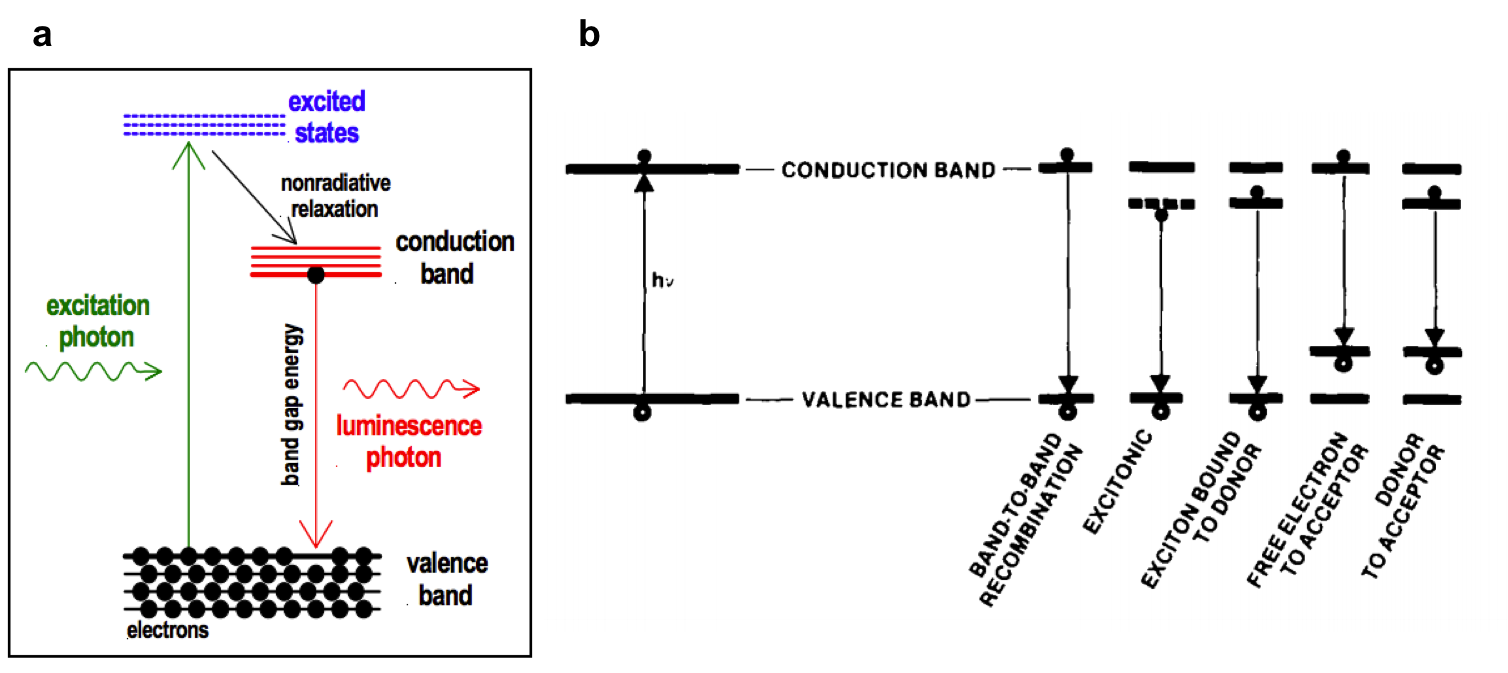
\includegraphics[width=1.0\textwidth]{figures/PL_transitions.png}
    \caption{Basic optical transitions involved in a measurement during photoluminescence spectroscopy (a). Common emission transitions detected during photoluminescence measurements, including transitions involving defect levels (b). Figures taken from reference \citenum{} and \citenum{Pankove} respectively.}
  \label{PL_transitions}
\end{figure}

Observed band tailing can be caused by either spatial band gap variations or electrostatic potential fluctuations in the material \cite{band_tail}. In the case of the latter, it is the inhomogenous distribution of ionized defects that cause the fluctuations. An ionized donor exerts and attractive force on conduction electrons and a repulsive force on valence holes. As the defects are distributed randomly, the local interaction varies depending on the crowding of the defects. In this case the energy gap between the valence band and conduction band is maintained, as shown in figure \ref{pankove_elec_fluc} and the states of each tail are spatially separated \cite{Pankove}. Defects can also result in fluctuations in the band gap of a material. For example, if an impurity atom is of a different size to the atoms of the host lattice, then this can result in a local mechanical strain, as shown in figure \ref{pankove_band_fluc}b which results in a deformation potential, such as that shown in figure \ref{pankove_band_fluc}c for an edge dislocation defect. Local strains can alter the separation of atoms in the crystal and, as figure \ref{pankove_band_fluc}a shows, the atomic separation within a crystal has a significant impact on the band structure.

\begin{figure}[h!]
  \centering
    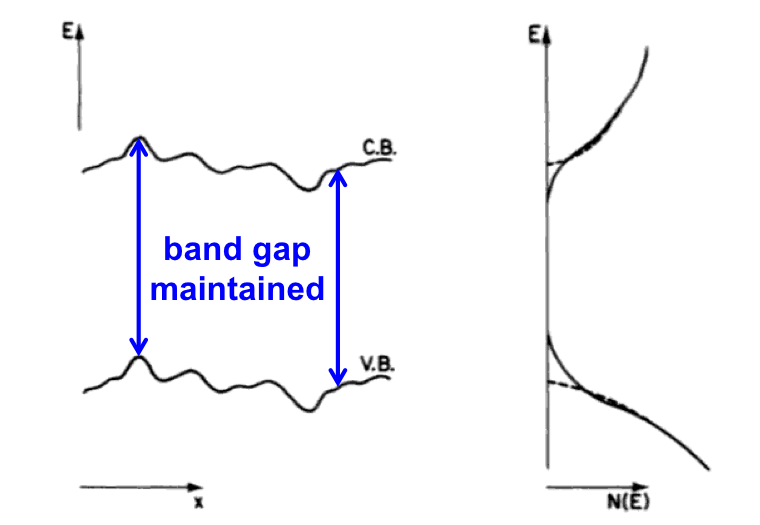
\includegraphics[width=0.6\textwidth]{figures/pankove_elec_fluc.png}
    \caption{The perturbation of the band edges by Coulomb interaction with inhomogeneously distributed impurities (left), leading to the formation of tail states (right). Dashed lined show the distribution of states in the unperturbed case. Figure taken from reference \citenum{Pankove}.}
  \label{pankove_elec_fluc}
\end{figure}

\begin{figure}[h!]
  \centering
    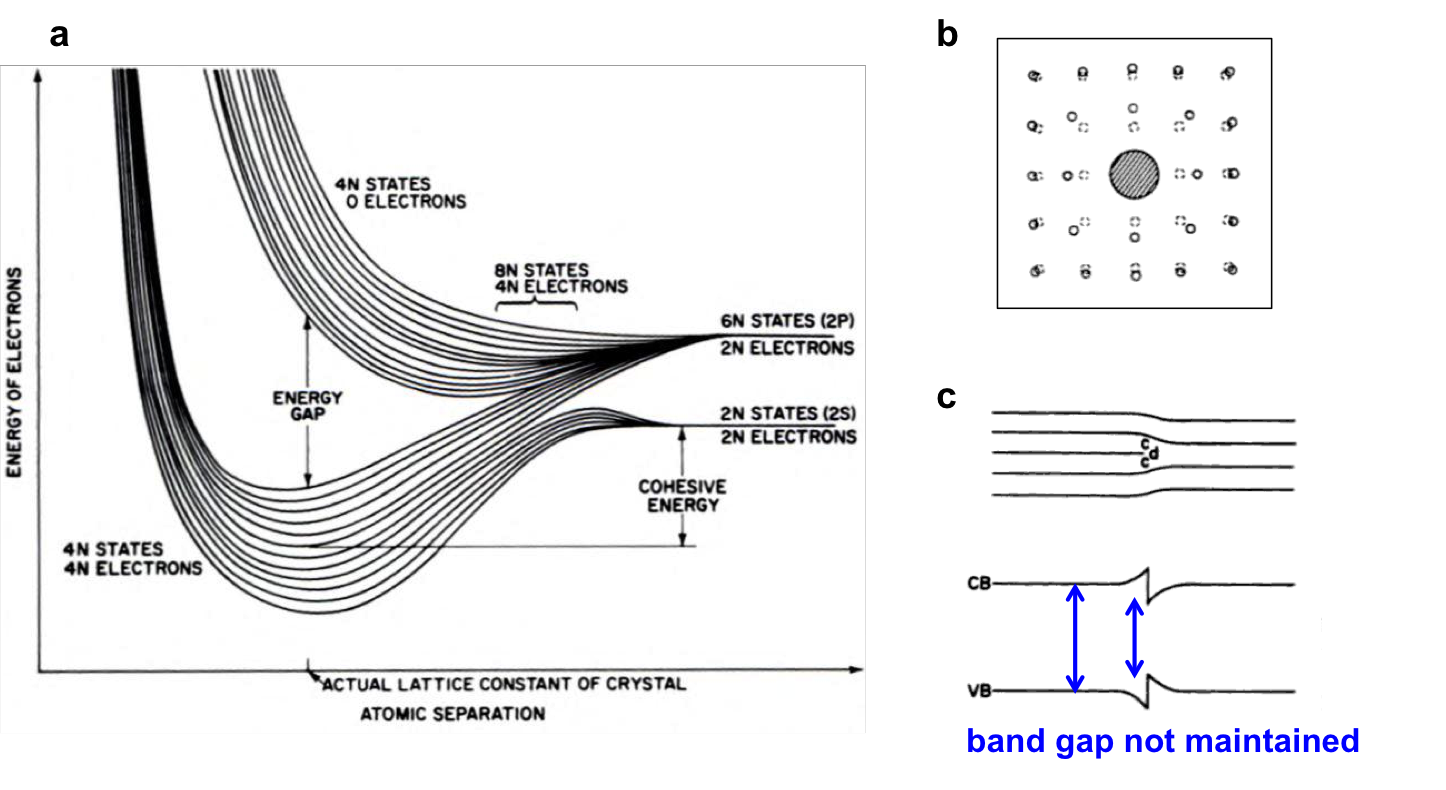
\includegraphics[width=1.0\textwidth]{figures/pankove_band_fluc.png}
    \caption{Energy banding of allowed levels in diamond as a function of spacing between atoms (a). Compressional strain induced in a crystal lattice by the incorporation of a large impurity atom (b). Deformation potential in the band structure due to compressional and dilational strain from an edge dislocation defect (c). Figures taken from reference \citenum{Pankove}.}
  \label{pankove_band_fluc}
\end{figure}


\subsection{Impact of Defects and Disorder on Solar Cell Performance}\label{defects_in_PV}

As already discussed, even very low concentrations of defects in a semiconductor can have a significant impact on its optoelectronic properties and therefore heavily influence the performance of an optoelectronic device composed of the material. As discussed in section \ref{current_tech}, one of the main motivations behind developing thin-film PV technologies, where the absorber layer is considerably thinner than that of a conventional silicon wafer, was to reduce the demand on the quality and low-defect concentrations of the material to reduce the energy intensity and high costs associated with the fabrication of the high quality material. A large number of compound semiconductors with direct band gaps have been studied for use in solar cells and some, such as CdTe and CIGSSe, have been commercialized. However, as the number of elemental components in a compound semiconductor increases, so does the various types of defects and disorder that can be present in the material, some of which will have more detrimental effects on device performance than others.\\

Firstly, thin-films of solar absorber materials fabricated using low cost synthesis techniques will be highly polycrystalline, therefore the layer will contain many grain boundaries, which can heavily influence device performance. In the specific case of CuInSe$_2$, the more polycrystalline material was found the produce higher-performing devices than its single crystalline counterpart \cite{CIS1_3, CIS1_4}, but this has been attributed to the unique grain boundary physics of this material \cite{CIS1, CIS2}. Typically, grain boundaries are a sink for defects and therefore are more closely associated with the detrimental effect of defects on PV performance, such as Shockley-Read-Hall recombination which will be discussed further below. 
It can also be very challenging to synthesise a single phase of a multicomponent material as a large number of secondary phases will also exist which can unintentionally be produced. For CZTS, phase diagrams have been constructed that show only a very narrow region for single phase CZTS, where only an absolute deviation of 1-2$\%$ in the composition at most would still result in a single phase of the crystal \cite{SandS}. A schematic showing various possible secondary phases that could be produced during the synthesis of CZTS is shown in figure \ref{CZTS_phase_diagram}. The formation of secondary phases can be problematic due to recombinations at interfaces between secondary phases but also because the different phases may have a different band gap. Some of which may be less than that of CZTS and so could hinder device performance.
However in our study, we are primarily concerned with the properties of the bulk material, to determine if there are fundamental material properties that will limit device performance.\\

\begin{figure}[h!]
  \centering
    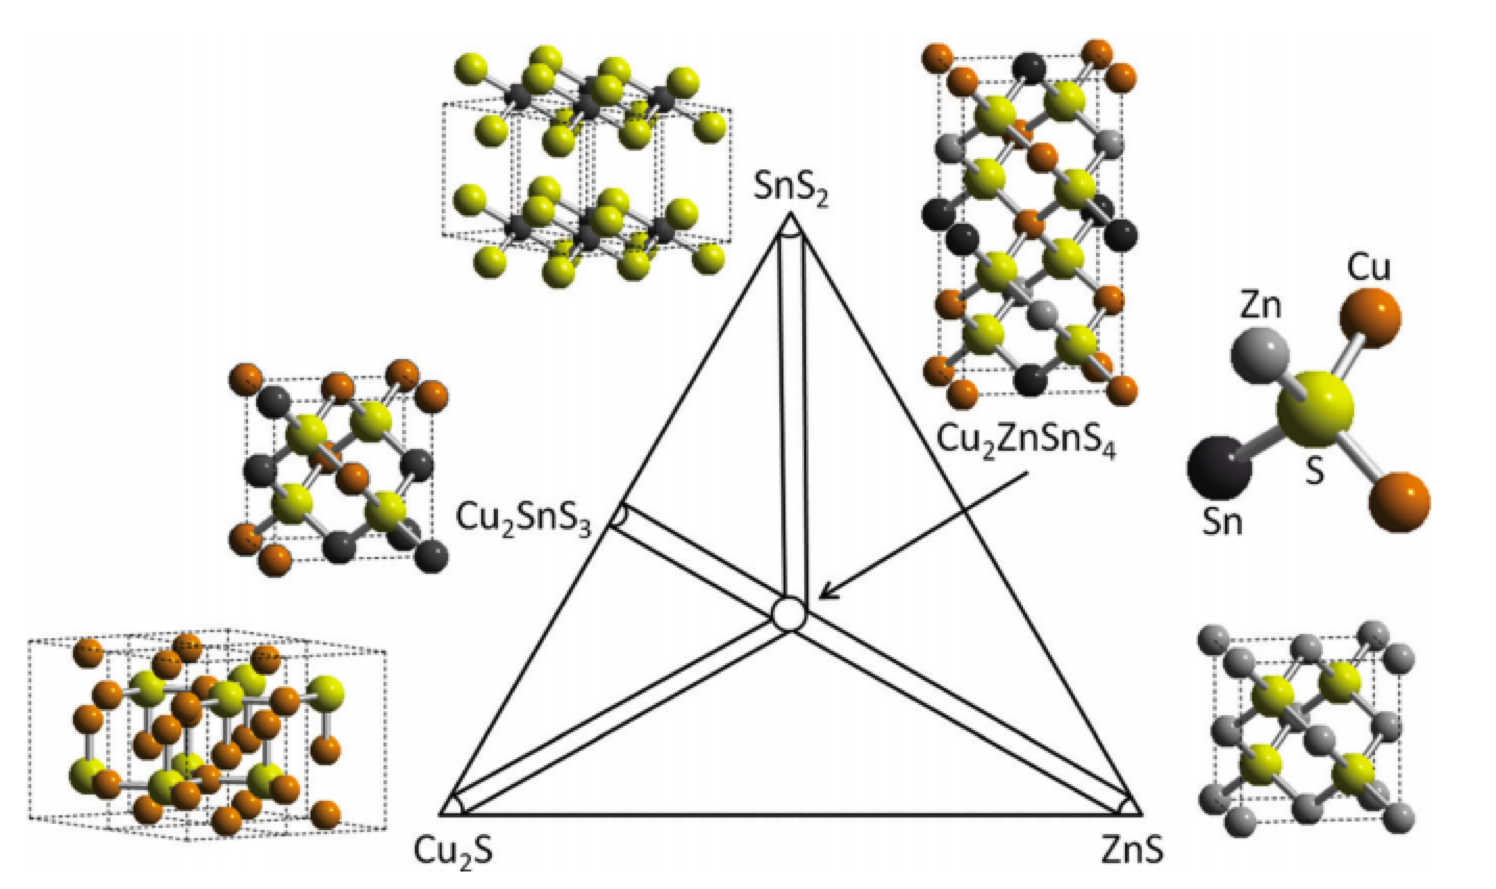
\includegraphics[width=0.8\textwidth]{figures/CZTS_phase_diagram.png}
    \caption{Schematic of the thin film
Cu$_2$S-ZnS-SnS$_2$ ternary phase diagram at 325$^{\circ}$C deposition temperature. The crystal structures of CZTS and the observed secondary phases are also presented. Figure taken from reference \citenum{CZTS_phase_diagram}.}
  \label{CZTS_phase_diagram}
\end{figure}

Of bulk defects and disorder, defects that produce mid-gap states (i.e. deep defect levels) act as Shockley-Read-Hall recombination sites \cite{SRH}, which was illustrated in figure \ref{SRH}. This is regarded as the most important recombination process in real, non-perfect semiconductors. It is a form of non-radiative recombination where a charge carrier is trapped in the defect state before recombining with a charge carrier of opposite polarity. This type of recombination is known to be detrimental to device performance as essentially  it results in energy input from sunlight not being converted into electricity \cite{Nelson4}.
In the case of {\CZTS}, for the most part predictions of defect formation energy and defect levels suggest that defects which would be expected to produce a deep defect level, also have a high formation energy so would be expected to be less likely to form \cite{defect1}.\\

For {\CZTS} a lot of attention in the literature has been paid to disorder amongst Cu and Zn cations with a large amount of experimental evidence for the presence of this disorder \cite{Schorr, CZTS_Xray, CZTS_TEM} and theoretical predictions for the low formation energy of the  $[Cu_{Zn}^{-} + Zn_{Cu}^{+}]$ \cite{defect1}.
During the synthesis of CZTS, temperatures above room temperature are used and it is possible for some of the thermal disorder associated with the system at higher temperatures to be `frozen in' to the material as it cools to room temperature.
Near resonant Raman spectroscopy has been used to examine thin films of CZTS prepared using different thermal treatments to determine if long post-annealing cooling times could produce films with a high level of order amongst Cu and Zn cations. However in this study, the authors postulate that achieving a very high level of order amongst Cu and Zn could require years \cite{Katharina}. This clearly wouldn't be a practical treatment for a PV device and so it would seem that the presence of a fairly large amount of disorder amongst Cu and Zn, and hence $Cu_{Zn}^{-}$ and $Zn_{Cu}^{+}$ antisites,  is inevitable in the material.\\

Although $Cu_{Zn}^{-}$ and $Zn_{Cu}^{+}$ antisite defects have been predicted to produce only shallow defect levels within the band gap of the material \cite{defect1}, their presence could be linked to band tailing in the material. 
Point defects in an otherwise perfect lattice can be regarded as missing lattice atoms, which are replaced by lattice defects. Therefore for every defect that creates one or more levels in the band gap of the material, the same number of levels that would have been created by the atoms in the host lattice are missing. Additionally, the lattice atoms surrounding the defect relax into shifted positions and also create states that could be shifted slightly into the band gap \cite{thin_film_Boer}. All of these states contribute to perturbations in the band edge, such as that shown in figure \ref{pankove_band_tailing}. Such a tail of band states into the band gap is often referred to as a Lifshitz tail \cite{Lifshitz1964}, it can be observed experimentally and is most noticeable in heavily doped and amorphous semiconductors \cite{thin_film_Boer}. For disorder due to defects with a correlation length on the order of interatomic spacing, the absorption coefficient, $\alpha_{0}$ (which was discussed as a key property for PV materials in section \ref{PV_properties}) shows a exponential decline. This effect is illustrated in figure \ref{urbach_fig}. This dependence of the optical absorption is widely observed in disordered semiconductors \cite{thin_film_Boer} and is referred to as the Urbach tail \cite{Urbach1953}. Such tailing can be quantified by the Urbach energy, and it has recently been proposed that there is a direct link between the Urbach energy and open circuit voltage deficit in standard photovoltaic materials \cite{culprit, UrbachE_Voc}.

\begin{figure}[h!]
  \centering
    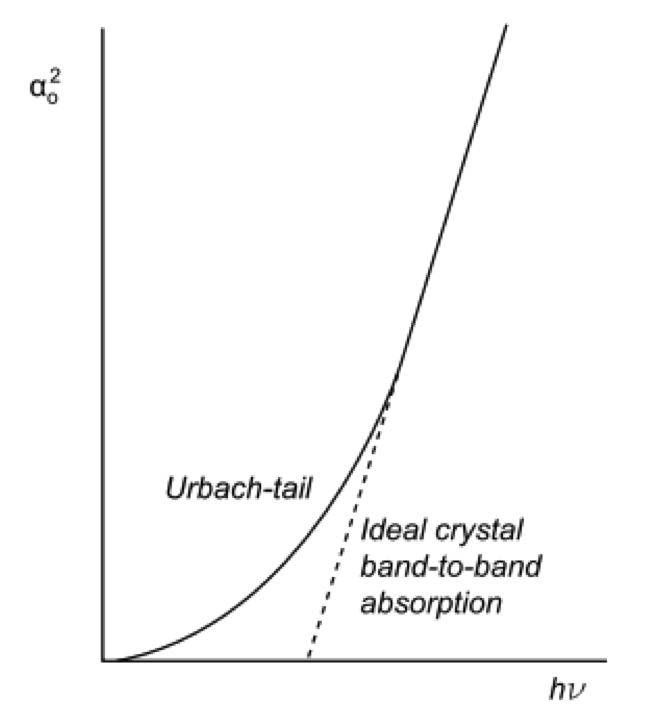
\includegraphics[width=0.6\textwidth]{figures/urbach_fig.png}
    \caption{Optical absorption spectrum of a typical direct band gap semiconductor with the absorption coefficient, $\alpha_{0}$, proportional to the extended density of states in the Urbach tail. Figure taken from reference \citenum{thin_film_Boer}.}
  \label{urbach_fig}
\end{figure}


\subsection{Photoluminescence Spectra of \CZTS}\label{CZTS_PL_section}
Photoluminescence (PL) spectroscopy is a popular method to inspect solar cell materials as it does not require a full functioning device and can be a powerful tool for probing defects in semiconductors. There are a large number of possible optical transitions that can be detected by PL measurements, some of which were illustrated in figure \ref{PL_transitions}. For this reason, low-temperature PL can be a particularly powerful tool for probing defects as energy level occupancy is dependent upon temperature and so not all PL recombinations will occur at the same temperature, allowing for the isolation of different types of recombination transitions \cite{spatial_resolved_book}. There are also other variations in the set up of a PL measurement that can be altered to provide more information on the band structure and how it is altered by the presence of defects. Firstly the intensity of the laser can be increased to determine if states are localized (such as those introduced by defects) or extended states (such as the conduction and valence bands) by if it is possible to saturate the states in the case of localized states such that an increase in laser intensity no longer increases the PL peak \cite{Gershon}. Secondly, time-resolved PL (TRPL) measurements  can be used to differentiate between recombination mechanisms with different carrier lifetimes. Slower optical transitions usually involve carriers in localized states, whereas faster transitions usually involve delocalized states \cite{Gershon}.\\

\begin{figure}[h!]
  \centering
    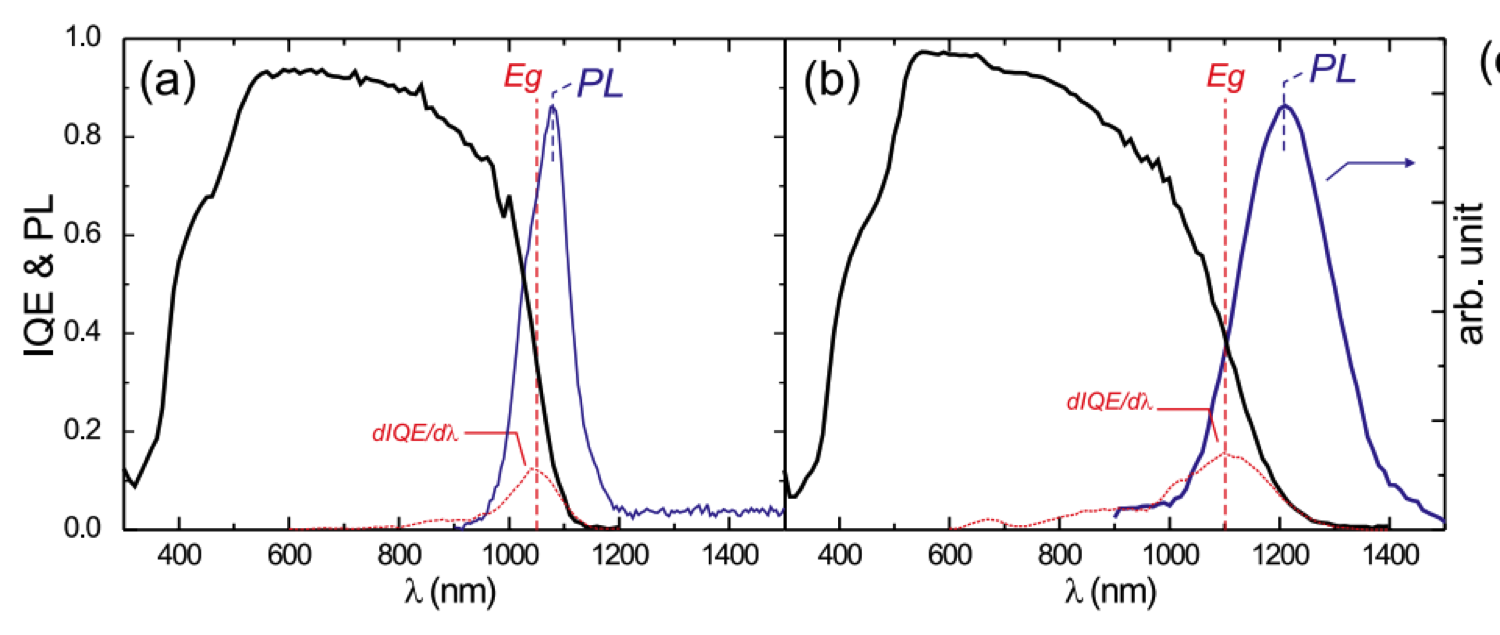
\includegraphics[width=1.0\textwidth]{figures/CZTS+CIGS_PL.png}
    \caption{The internal quantum efficiency (IQE), band gap as determined from the IQE inflection point and the photoluminescence spectra of high performance devices with thin-film absorber layers of (a) CIGSSe (E$_g$ = 1.19 eV) and ) CZTSSe (E$_g$ = 1.13 eV). Figure taken from reference \citenum{band_tail}.}
  \label{CZTS+CIGS_PL}
\end{figure}

Several PL studies have been performed on kesterite-structured samples of {\CZTS}, Cu$_2$ZnSnSe$_4$ and alloys of the two. PL measurements have been performed on both full devices and polycrystalline thin-films \cite{band_tail, Gershon, Gershon_ref18, Romero, Miyamoto, Unold} and single crystals \cite{Halliday, Levcenko, Hones}. In addition studies such as reference \citenum{Halliday} compare the PL spectra for varying compositions of the sample, whereas in reference \citenum{band_tail} measurements on both CIGSSe and CZTSSe thin films are performed in an attempt to account for the difference in the performance of these two technologies by comparing their defect-influenced PL emission spectra. Polycrystalline samples are more similar to those likely to be used in thin-film CZTS photovoltaic devices, however comparison between those measurements with single crystal measurements could enable the isolation of recombination at grain boundaries from those due to bulk defects. Also measurements performed on single crystals as close to perfectly stoichiometric {\CZTS} as possible are likely to be the most directly relatable to our simulations on bulk systems. However one feature common to all of the PL spectra from studies on kesterite samples is clear evidence of defects and disorder from the observed band tailing. The PL spectra of kesterite samples usually features a much broader peak than that observed in CIGSSe samples, such as that shown in figure \ref{CZTS+CIGS_PL}. The energy of the maximum PL peaks of kesterite samples is also usually considerably red-shifted compared to the energy of the band gap. These two features are usually attributed to band tailing caused by either spatial band gap variations or electrostatic potential fluctuations in the absorber material, which were discussed in section \ref{PL_section}.  Both effects lead to a non-zero density of states (DOS) within the band gap \cite{culprit, band_tail}. 
Measurements performed in reference \citenum{band_tail} found the tailing in CZTSSe to be roughly twice as severe as that observed in higher-performing CIGSSe devices.\\

%\cite{band_tail} = Mitzi PL paper, \cite{Gershon} = first paper in overview, \cite{Gershon_ref18} = previous work with good overview of PL

However, there is some disagreement in the literature about the main recombination mechanisms that could explain the observed PL spectra. Of the measurements performed on single crystals, reference \citenum{Levcenko} perform measurements on near-stoichiometric CZTS crystals and report a free-to-bound transition between the conduction band and an acceptor level. In reference \citenum{Hones}, donor-acceptor-pair (DAP) transitions are reported for large single grains of CZTS, whereas in reference \citenum{Halliday} where measurements are performed on CZTS single-crystals of varying composition, they report PL measurements through spatially fluctuating band states as would be expected from either spatial band gap variations or electrostatic potential fluctuations from heavy defect compensation. Therefore in bulk monograins of CZTS PL band-to-impurity, DAP and spatially fluctuating band-type recombinations have all been reported and the exact sources, or rather associated defects, for these recombination mechanisms are not yet known \cite{Gershon_ref18}.\\

For measurements performed on polycrystalline kesterite samples, some studies attribute the spectra to spatially fluctuating band tail states \cite{Romero}, whereas others suggest that recombination in CZTS is dominated by the distinct energy levels introduced by DAPs \cite{Unold, Miyamoto}. In other studies, an explanation that is almost a combination of the two is proposed \cite{Gershon, Gershon_ref18}. These studies refer to a quasi-donor-acceptor-pair (QDAP) model, where the word `quasi' is used to indicate a deviation from the classical DAP model for recombinations, such as that shown in figure \ref{PL_transitions}, due to interactions between defects. In reference \citenum{Gershon_ref18} they note that distinguishing between DAP recombination and spatially fluctuating band tails caused by spatially varying densities of ionized donor and acceptor defects is particularly complicated as a high density of compensating DAPs is necessarily co-incident with spatial fluctuation in electrostatic potential. In the same work, they note that the dominance of donor and acceptor pairs on PL spectra is in agreement with theoretical predictions such as those by Chen et al shown in figure \ref{Chen_cluster1} \cite{defect1} that antisite DAPs such as $[Cu_{Zn}^{-} + Zn_{Cu}^{+}]$ should be abundant due to the low formation energy of the defect complex and also experimental observations of cation disorder by neutron diffraction, synchrotron radiation x-ray diffraction and aberration corrected scanning transmission electron microscopy respectively \cite{Schorr, CZTS_Xray, CZTS_TEM}.\\

In this work we begin two studies on defects in {\CZTS}. Firstly, we will attempt to quantify the contribution to the observed band tailing in CZTS from disorder amongst copper and zinc cations, or equivalently, the presence of $[Cu_{Zn}^{-} + Zn_{Cu}^{+}]$ antisite defect pairs. The methodology will be outlined in more detail in section \ref{MC_section}, but the general approach will be to use Monte Carlo simulations that have been parameterised with first-principles calculations to determine the extent of Cu-Zn disorder in CZTS at various temperatures and to then study the distribution of electrostatic potential across the system from the inhomogeneous spatial arrangement of the charged antisite defects,  $Cu_{Zn}^-$ and $Zn_{Cu}^+$.
Secondly we have begun a study to re-examine the formation energy of sulfur vacancies as they have been predicted \cite{defect1} to result in a mid gap state, but it is possible that the formation energy may have been overestimated when typical synthesis conditions are taken into account. This will be discussed further as future work in section \ref{Vs_proj}.





%\subsection{Modulation Spectroscopy \& Band Gap Broadening}
%See pdf from Laurie - method used by PVTEAM to measure band gap broadening of CZTS single crystal + see quantum processes in semiconductors pg 244




%\section{Novel Optoelectronic Phenomena for High Performance Solar Cells}


%\subsection{Spin Orbit Interaction \& Rashba Splitting}\label{SOC_section}
%Refer to: pg 13 + 21-22 \cite{Bechstedt} + quantum processes in semiconductors pg 13 for SOC\\

% see webpages: pg 84 for discussion of effect of SOC on lattice without inversion symmetry!  + useful slide

%Look for textbook source?

%See rashba splitting paper (pre-Duke visit papers)

%\subsection{Photovoltaic-Ferroelectric Phenomena}\label{FE_PV_section}

%Ferroelectric PV materials are currently receiving a great deal of research interest, however the origin of their PV properties are considered to be unresolved \cite{Rappe}. A large number of theories have been proposed in an attempt to explain the two observed ferroelectric-photovoltaic (FE-PV) phenomena: the bulk PV effect (BPE), also referred to as the photogalvanic effect, and the anomalous PV effect (APE). In the BPE, a direct current appears in a homogeneous medium under uniform illumination and this can occur in all materials without a center of symmetry  \cite{PGE}. Ferroelectric materials exhibit this effect strongly \cite{Rappe} and the first observation of this effect was in 1956 with photovoltages measured in un-doped single crystals of the ferroelectric material BaTiO$_3$ \cite{keith_46}. In the case of the APE, photovoltages have been measured that are orders of magnitude larger than the band gap of the material \cite{keith_54}, but has been observed to disappear when the sample undergoes a phase transition to a paraelectric phase \cite{nonlinear_dielectric}, and so no longer exhibits spontaneous electric polarization. Theories have been developed to explain the FE-PV phenomena based around experimental observations of factors that have been shown to influence the photovoltage of FE-PV devices, such as:  the distance between the two opposite electrodes \cite{rev_28,rev_46}, intensity of incident light \cite{rev_47}, electrical conductivity \cite{Fridkin}, remnant polarization of the
%ferroelectric crystals \cite{rev_48}, crystallographic orientation \cite{rev_49}, the dimension or size of the crystals \cite{rev_46, rev_50}, domain walls \cite{rev_30} and the interface between the FE material and the electrode \cite{rev_37}.\\

%Models have been proposed to explain the BPE in ferroelectric materials based upon the built-in asymmetry of non-centrosymmetric crystals. One model is based on asymmetric scattering centres in the materials \cite{PGE}. In non-centrosymmetric crystals, the rate of the generation of charge carriers with momenta $\pm$k can be different due to asymmetric electron-hole scattering. A `ballistic current' can then be generated due to the momentum imbalance \cite{shift_current}.
%Another model, the shift current model \cite{shift_current}, has been proposed, which is based on the asymmetry of the electron density \cite{keith}.
%Light-induced transitions of charge carriers between bands in reciprocal space are accompanied by asymmetrical shifts in real space between atoms in elementary cells \cite{shift_current}.
%Such currents have been demonstrated for a number of materials, such as GaAs \cite{keith_52} and BiFeO$_3$, where this has been demonstrated using both computational \cite{keith_25} and experimental \cite{keith_51} techniques. \\

%The domain wall theory has been proposed to explain the large generated photovoltages in the APE \cite{domain_wall} and the Schottky-junction effect \cite{schottky_effect} and depolarization field model \cite{screen_effect, depol_model}, also referred to as the screening effect, have been proposed as additional contributions to the large photovoltage. Unlike the BPE, some theories to explain the APE rely on the nano- and microstructure of the material \cite{keith}. The latter two theories are related to the interface between the FE material and an electrode in a FE-PV device, but were originally neglected as the contributions to the photovoltage were believed to be small. However, these effects become more significant in thin-film devices where photovoltages are typically low \cite{FE_PV_rev1}, and thin-films are particularly relevant for PV applications.\\

%The domain wall theory was developed to explain observations of photovoltages in thin films of BiFeO$_3$ increasing linearly with the total number of ferroelectric domain walls along the net direction of electric polarization and vanishing along the direction perpendicular to the net polarization \cite{rev_30}. In this theory, the narrow ferroelectric domain walls drive the dissociation of photogenerated excitons and so  act as nanoscale photovoltage generators connected in series. The photocurrent across the domain walls is therefore continuous but the photogenerated voltage accumulates along the direction of net polarization, allowing for photovoltages that are considerably larger than the band gap of the material \cite{FE_PV_rev1}.
%In the Schottky-junction effect, the FE semiconductor forms a Schottky contact with the metal electrodes, which then generate a photocurrent under illumination due to the local electric field caused by the band bending near to the electrode. This photocurrent is dependent upon the Schottky barrier height and depletion region depth, but the photovoltage is still limited to the band gap of the material. Further, the additional photovoltage contribution from this effect can be cancelled out if the same electrode contacts are used, due to the opposite polarization of the two Schottky-junctions \cite{FE_PV_rev1}.
%In the depolarization field model, high densities of polarization charges are believed to accumulate on surfaces of polarized FE films, this then induces a large electric field inside the FE layer if the charge is not screened. This effect will be far more pronounced in a thin-film device. The electric field is thought to not be fully screened by the free charges in the metal or semiconductor that the FE layer is in contact with, resulting in a depolarization field. This depolarization field will be larger when the FE material has a large remnant electric polarization, the FE layer is thinner and when it is in contact with a semiconductor, as opposed to a metal, due to fewer free charge carriers and higher dielectric constant in a semiconductor than a metal, giving weaker screening. The depolarization field is believed to be the dominating force for the separation of photogenerated charge carrier pairs \cite{FE_PV_rev1}.\\

%Clearly the exact mechanism behind the observed PV phenomena in FE materials are not yet fully understood, but they could open up new possible routes for materials to enable higher performance solar cells. In particular, the APE could be utilized for materials with higher V$_{OC}$ to enable a higher power output from a solar cell. Additionally, it has been suggested that ferroelectric domains may be able to drive the separation of photoexcited electron-hole pairs to reduce detrimental recombination in solar absorber materials \cite{Jarv}. 